\documentclass[tikz,border=10pt]{standalone}
\begin{document}
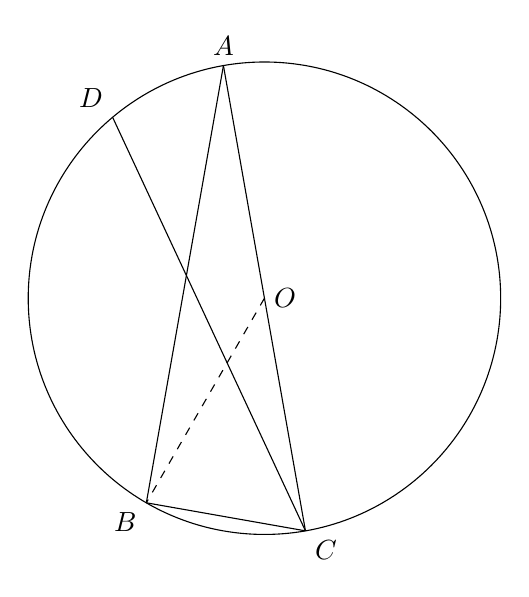
\begin{tikzpicture}
  \coordinate (O) at (0,0);
  \coordinate (A) at (100:3);
  \coordinate (C) at (280:3);
  \coordinate (B) at (240:3);
  \coordinate (D) at (130:3);

  \draw (O) circle (3);
  \draw (A) -- (B);
  \draw (B) -- (C);
  \draw (A) -- (C);
  \draw (D) -- (C);
  \draw[dashed] (O) -- (B);

  \node[above] at (A) {$A$};
  \node[below left] at (B) {$B$};
  \node[below right] at (C) {$C$};
  \node[above left] at (D) {$D$};
  \node[right] at (O) {$O$};
\end{tikzpicture}
\end{document}
